%=====================================================================
%  00-CONTOH-FITUR.TEX — SLIDE PANDUAN & CONTOH PEMAKAIAN TEMPLATE
%=====================================================================
%  File ini adalah "buku saku hidup": setiap slide memperagakan satu
%  fitur template BERSERTA komentar kode sumbernya. Slide ini tetap
%  diikutkan pada PDF hasil kompilasi sebagai dokumentasi; beri tanda
%  % pada baris %=====================================================================
%  00-CONTOH-FITUR.TEX — SLIDE PANDUAN & CONTOH PEMAKAIAN TEMPLATE
%=====================================================================
%  File ini adalah "buku saku hidup": setiap slide memperagakan satu
%  fitur template BERSERTA komentar kode sumbernya. Slide ini tetap
%  diikutkan pada PDF hasil kompilasi sebagai dokumentasi; beri tanda
%  % pada baris %=====================================================================
%  00-CONTOH-FITUR.TEX — SLIDE PANDUAN & CONTOH PEMAKAIAN TEMPLATE
%=====================================================================
%  File ini adalah "buku saku hidup": setiap slide memperagakan satu
%  fitur template BERSERTA komentar kode sumbernya. Slide ini tetap
%  diikutkan pada PDF hasil kompilasi sebagai dokumentasi; beri tanda
%  % pada baris %=====================================================================
%  00-CONTOH-FITUR.TEX — SLIDE PANDUAN & CONTOH PEMAKAIAN TEMPLATE
%=====================================================================
%  File ini adalah "buku saku hidup": setiap slide memperagakan satu
%  fitur template BERSERTA komentar kode sumbernya. Slide ini tetap
%  diikutkan pada PDF hasil kompilasi sebagai dokumentasi; beri tanda
%  % pada baris \input{00-contoh-fitur} di main.tex saat presentasi.
%
%  TIPS: untuk menuliskan nama perintah/kode di dalam teks, gunakan
%  \code{...} (makro bawaan ppt.sty) — contoh \code{\frac{a}{b}}.
%=====================================================================

%---------------------------------------------------------------------
%  CONTOH 1 — STRUKTUR DASAR SLIDE & TEKS
%---------------------------------------------------------------------
\section{PANDUAN PENGGUNAAN}

\begin{frame}
    \frametitle{Cara Membuat Slide Baru}   % judul yang tampil di batang atas

    % --- Struktur minimum sebuah slide ----------------------------
    %  \begin{frame}
    %      \frametitle{Judul Slide Anda}
    %      isi slide ...
    %  \end{frame}
    %  Letakkan \section{NAMA BAGIAN} SEBELUM \begin{frame} agar
    %  slide masuk ke navigasi atas dan slide OUTLINE.

    \begin{columns}[T]          % [T] = rata atas antar kolom
        \begin{column}{0.48\textwidth}   % lebar kolom (48% teks)
            \begin{block}{Penekanan teks}
                \footnotesize
                \begin{itemize}
                    \item \textbf{tebal}  : \code{\textbf{tebal}}
                    \item \textit{miring} : \code{\textit{miring}}
                    \item \alert{merah}   : \code{\alert{merah}}
                    \item \textcolor{telu}{merah Telkom}:\\
                          \code{\textcolor{telu}{...}}
                \end{itemize}
            \end{block}
        \end{column}

        \begin{column}{0.48\textwidth}
            \begin{block}{Ukuran font \& perataan}
                \footnotesize
                \begin{itemize}
                    \item[\textcolor{scisGold}{$\Rightarrow$}] Urut kecil:
                          \code{\tiny < \small < \normalsize}
                    \item[\textcolor{scisGold}{$\Rightarrow$}] Rata kiri-kanan:
                          tulis \code{\justifying} (paket ragged2e)
                    \item[\textcolor{scisGold}{$\Rightarrow$}] Daftar bertingkat:
                          \code{\item} di dalam \code{\item}
                    \item[\textcolor{scisGold}{$\Rightarrow$}] Panah khusus:
                          \code{\item[$\Rightarrow$]}
                \end{itemize}
            \end{block}
        \end{column}
    \end{columns}
\end{frame}

%---------------------------------------------------------------------
%  CONTOH 2 — GAMBAR, TABEL & PERSAMAAN
%---------------------------------------------------------------------
\begin{frame}
    \frametitle{Memasukkan Gambar, Tabel \& Persamaan}
    \begin{columns}[T]
        \begin{column}{0.46\textwidth}
            % --- GAMBAR + CAPTION + LABEL -----------------------------
            %  \label wajib UNIK; rujuk dengan Gambar~\ref{fig:contoh}
            \begin{figure}
                \centering
                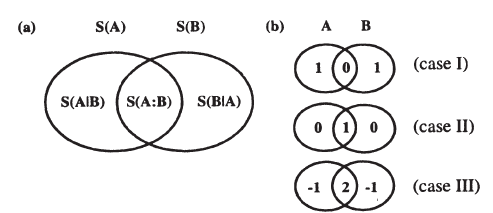
\includegraphics[width=0.9\textwidth]{gambar/DIAGRAM/diagram2.png}
                \captionsetup{font=tiny, justification=justified}
                \captionof{figure}{Contoh caption: diagram entropi sistem
                dua-qubit. Nomor otomatis \textit{slide.urutan}.}
                \label{fig:contoh}
            \end{figure}
            {\tiny Rujuk dengan
            \code{Gambar~\ref{fig:contoh}} $\rightarrow$
            Gambar~\ref{fig:contoh}.}
        \end{column}

        \begin{column}{0.52\textwidth}
            % --- TABEL PROFESIONAL (booktabs) --------------------------
            \begin{table}
                \centering
                {\tiny
                \begin{tabular}{llc}
                    \toprule                              % garis atas
                    \textbf{Perintah} & \textbf{Hasil} & \textbf{Ket.} \\
                    \midrule                              % garis tengah
                    \code{\sigma_x} & $\sigma_x$ & Pauli-X \\
                    \code{\otimes}   & $\otimes$  & tensor  \\
                    \code{\dagger}   & $\dagger$  & adjoint \\
                    \bottomrule                           % garis bawah
                \end{tabular}}
                \captionof{table}{Contoh tabel \textit{booktabs}.}
                \label{tab:contoh}
            \end{table}

            % --- PERSAMAAN BERLABEL ------------------------------------
            %  \label{eq:...} lalu rujuk: Persamaan~\ref{eq:vonneumann}
            \begin{equation}
                S(\rho) = -\Tr\!\left(\rho \log \rho\right)
                \label{eq:vonneumann}
            \end{equation}
            {\tiny Persamaan~\ref{eq:vonneumann} = entropi von Neumann.}
        \end{column}
    \end{columns}
\end{frame}

%---------------------------------------------------------------------
%  CONTOH 3 — NOTASI KUANTUM (DIRAC) & TULISAN MATEMATIKA
%---------------------------------------------------------------------
%  Makro notasi tersedia di ppt.sty bagian [8]; paket braket menyediakan
%  \ket, \bra, \Braket. Prinsip penulisan:
%    * vektor keadaan selalu \ket{...}   ->  |psi>
%    * dual (transpose konjugat) \bra{...}
%    * proyektor \ketbra{a}{b}           ->  |a><b|
%    * operator ditandai "topi": \hat{U}
\begin{frame}
    \frametitle{Cheatsheet Notasi Kuantum}
    \begin{columns}[T]
        \begin{column}{0.48\textwidth}
            {\small\textbf{Keadaan \& operator}}
            {\tiny
            \begin{itemize}\justifying
                \item[$\Rightarrow$] Qubit:
                      $\ket{0}=\begin{bmatrix}1\\0\end{bmatrix}$,
                      $\ket{1}=\begin{bmatrix}0\\1\end{bmatrix}$
                \item[$\Rightarrow$] Superposisi:
                      $\ket{\psi}=\alpha\ket{0}+\beta\ket{1}$,
                      $|\alpha|^2+|\beta|^2=1$
                \item[$\Rightarrow$] Bell/EPR:
                      $\ket{\psi_{AB}}=\tfrac{1}{\sqrt{2}}(\ket{00}+\ket{11})$
                \item[$\Rightarrow$] Proyektor: $\ketbra{0}{0}$,
                      $\ketbra{1}{1}$
                \item[$\Rightarrow$] Operator: $\hat{U}\hat{U}^\dagger=\hat{I}$
            \end{itemize}}
        \end{column}
        \begin{column}{0.48\textwidth}
            {\small\textbf{Matriks densitas \& entropi}}
            {\tiny
            \begin{itemize}\justifying
                \item[$\Rightarrow$] Campuran:
                      $\rho=\sum_i p_i\,\ketbra{\psi_i}{\psi_i}$
                \item[$\Rightarrow$] Matriks gabungan:
                      $\rho_{AB}=\rho_A\otimes\rho_B$
                \item[$\Rightarrow$] Jejak (trace):
                      $\Tr(\rho)=1$;
                      $\Tr_B(\rho_{AB})=\rho_A$
                \item[$\Rightarrow$] Entropi:
                      $S(\rho)=-\Tr(\rho\log\rho)$
                \item[$\Rightarrow$] Kondisional:
                      $S(A|B)=S(AB)-S(B)$ (bisa negatif!)
            \end{itemize}}
        \end{column}
    \end{columns}
\end{frame}

%---------------------------------------------------------------------
%  CONTOH 4 — MENULIS KODE PROGRAM (LISTINGS)
%---------------------------------------------------------------------
\begin{frame}[fragile]   % [fragile] WAJIB jika slide berisi lstlisting
    \frametitle{Menampilkan Kode Program}
    \begin{columns}[T]
        \begin{column}{0.48\textwidth}
            {\tiny Gaya kode diatur di \code{ppt.sty} bagian [7].
                   Selalu tambahkan opsi \code{[fragile]} pada frame
                   yang memuat \code{lstlisting}.}
            \begin{lstlisting}[language=Python,basicstyle=\ttfamily\scriptsize]
# Contoh simulasi qubit (Python)
import numpy as np
I = np.eye(2)          # matriks identitas
X = np.array([[0, 1],
              [1, 0]]) # Pauli-X
rho = 0.5*(I + X)      # matriks densitas
print(np.trace(rho))   # Tr(rho) = 1
            \end{lstlisting}
        \end{column}
        \begin{column}{0.48\textwidth}
            \begin{lstlisting}[language=Matlab,basicstyle=\ttfamily\scriptsize]
% Contoh kanal depolarizing (MATLAB)
p  = 0.05;              % prob. depolarisasi
I2 = eye(2);
rho_i = [0.5 0; 0 0.5];
rho  = p*(I2/2) + (1-p)*rho_i;
            \end{lstlisting}
            {\tiny Kode inline: gunakan \code{\code{...}},
                   contoh: \code{np.trace(rho)}.}
        \end{column}
    \end{columns}
\end{frame}

%---------------------------------------------------------------------
%  CONTOH 5 — KUTIPAN, FOOTNOTE & BLOK
%---------------------------------------------------------------------
\begin{frame}
    \frametitle{Kutipan Pustaka \& Blok Informasi}
    \begin{columns}[T]
        \begin{column}{0.48\textwidth}
            \begin{exampleblock}{Kutipan dari bib.bib}
                {\small
                \begin{itemize}\justifying
                    \item Nomor biasa: entropi kuantum
                          \cite{barnett2009quantum}.
                    \item Footnote lengkap (pertama kali):\
                          lihat catatan kaki bawah slide.
                    \item Footnote ringkas (kutipan berikutnya):\
                          juga di catatan kaki.
                \end{itemize}}
            \end{exampleblock}
            {\tiny Entri pustaka ditulis di \code{bib.bib}.}
        \end{column}
        \begin{column}{0.48\textwidth}
            \begin{alertblock}{Alert block --- hal penting}
                {\small Dipakai untuk peringatan/kesimpulan kunci.}
            \end{alertblock}
            \begin{block}{Block biasa}
                {\small Definisi, catatan, atau langkah analisis.}
            \end{block}
            {\tiny Footnote biasa juga bisa: teks\footnote{Contoh
                   footnote langsung tanpa berkas pustaka.}}
        \end{column}
    \end{columns}
    % CATATAN PENTING: footnote/citasi ber-footnote (irstcite dsb.)
    % dipanggil di LEVEL FRAME (di luar columns) agar lebarnya terpotok
    % dan tidak meluber keluar slide.
    \vspace{-0.1cm}{\tiny \firstcite{cerf1997negative};
     kutip ulang \secondcite{cerf1997negative}.}
\end{frame}
 di main.tex saat presentasi.
%
%  TIPS: untuk menuliskan nama perintah/kode di dalam teks, gunakan
%  \code{...} (makro bawaan ppt.sty) — contoh \code{\frac{a}{b}}.
%=====================================================================

%---------------------------------------------------------------------
%  CONTOH 1 — STRUKTUR DASAR SLIDE & TEKS
%---------------------------------------------------------------------
\section{PANDUAN PENGGUNAAN}

\begin{frame}
    \frametitle{Cara Membuat Slide Baru}   % judul yang tampil di batang atas

    % --- Struktur minimum sebuah slide ----------------------------
    %  \begin{frame}
    %      \frametitle{Judul Slide Anda}
    %      isi slide ...
    %  \end{frame}
    %  Letakkan \section{NAMA BAGIAN} SEBELUM \begin{frame} agar
    %  slide masuk ke navigasi atas dan slide OUTLINE.

    \begin{columns}[T]          % [T] = rata atas antar kolom
        \begin{column}{0.48\textwidth}   % lebar kolom (48% teks)
            \begin{block}{Penekanan teks}
                \footnotesize
                \begin{itemize}
                    \item \textbf{tebal}  : \code{\textbf{tebal}}
                    \item \textit{miring} : \code{\textit{miring}}
                    \item \alert{merah}   : \code{\alert{merah}}
                    \item \textcolor{telu}{merah Telkom}:\\
                          \code{\textcolor{telu}{...}}
                \end{itemize}
            \end{block}
        \end{column}

        \begin{column}{0.48\textwidth}
            \begin{block}{Ukuran font \& perataan}
                \footnotesize
                \begin{itemize}
                    \item[\textcolor{scisGold}{$\Rightarrow$}] Urut kecil:
                          \code{\tiny < \small < \normalsize}
                    \item[\textcolor{scisGold}{$\Rightarrow$}] Rata kiri-kanan:
                          tulis \code{\justifying} (paket ragged2e)
                    \item[\textcolor{scisGold}{$\Rightarrow$}] Daftar bertingkat:
                          \code{\item} di dalam \code{\item}
                    \item[\textcolor{scisGold}{$\Rightarrow$}] Panah khusus:
                          \code{\item[$\Rightarrow$]}
                \end{itemize}
            \end{block}
        \end{column}
    \end{columns}
\end{frame}

%---------------------------------------------------------------------
%  CONTOH 2 — GAMBAR, TABEL & PERSAMAAN
%---------------------------------------------------------------------
\begin{frame}
    \frametitle{Memasukkan Gambar, Tabel \& Persamaan}
    \begin{columns}[T]
        \begin{column}{0.46\textwidth}
            % --- GAMBAR + CAPTION + LABEL -----------------------------
            %  \label wajib UNIK; rujuk dengan Gambar~\ref{fig:contoh}
            \begin{figure}
                \centering
                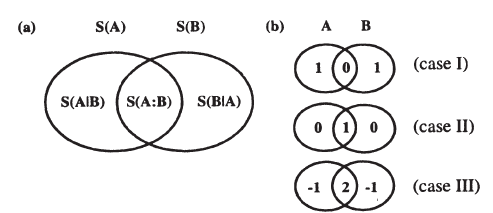
\includegraphics[width=0.9\textwidth]{gambar/DIAGRAM/diagram2.png}
                \captionsetup{font=tiny, justification=justified}
                \captionof{figure}{Contoh caption: diagram entropi sistem
                dua-qubit. Nomor otomatis \textit{slide.urutan}.}
                \label{fig:contoh}
            \end{figure}
            {\tiny Rujuk dengan
            \code{Gambar~\ref{fig:contoh}} $\rightarrow$
            Gambar~\ref{fig:contoh}.}
        \end{column}

        \begin{column}{0.52\textwidth}
            % --- TABEL PROFESIONAL (booktabs) --------------------------
            \begin{table}
                \centering
                {\tiny
                \begin{tabular}{llc}
                    \toprule                              % garis atas
                    \textbf{Perintah} & \textbf{Hasil} & \textbf{Ket.} \\
                    \midrule                              % garis tengah
                    \code{\sigma_x} & $\sigma_x$ & Pauli-X \\
                    \code{\otimes}   & $\otimes$  & tensor  \\
                    \code{\dagger}   & $\dagger$  & adjoint \\
                    \bottomrule                           % garis bawah
                \end{tabular}}
                \captionof{table}{Contoh tabel \textit{booktabs}.}
                \label{tab:contoh}
            \end{table}

            % --- PERSAMAAN BERLABEL ------------------------------------
            %  \label{eq:...} lalu rujuk: Persamaan~\ref{eq:vonneumann}
            \begin{equation}
                S(\rho) = -\Tr\!\left(\rho \log \rho\right)
                \label{eq:vonneumann}
            \end{equation}
            {\tiny Persamaan~\ref{eq:vonneumann} = entropi von Neumann.}
        \end{column}
    \end{columns}
\end{frame}

%---------------------------------------------------------------------
%  CONTOH 3 — NOTASI KUANTUM (DIRAC) & TULISAN MATEMATIKA
%---------------------------------------------------------------------
%  Makro notasi tersedia di ppt.sty bagian [8]; paket braket menyediakan
%  \ket, \bra, \Braket. Prinsip penulisan:
%    * vektor keadaan selalu \ket{...}   ->  |psi>
%    * dual (transpose konjugat) \bra{...}
%    * proyektor \ketbra{a}{b}           ->  |a><b|
%    * operator ditandai "topi": \hat{U}
\begin{frame}
    \frametitle{Cheatsheet Notasi Kuantum}
    \begin{columns}[T]
        \begin{column}{0.48\textwidth}
            {\small\textbf{Keadaan \& operator}}
            {\tiny
            \begin{itemize}\justifying
                \item[$\Rightarrow$] Qubit:
                      $\ket{0}=\begin{bmatrix}1\\0\end{bmatrix}$,
                      $\ket{1}=\begin{bmatrix}0\\1\end{bmatrix}$
                \item[$\Rightarrow$] Superposisi:
                      $\ket{\psi}=\alpha\ket{0}+\beta\ket{1}$,
                      $|\alpha|^2+|\beta|^2=1$
                \item[$\Rightarrow$] Bell/EPR:
                      $\ket{\psi_{AB}}=\tfrac{1}{\sqrt{2}}(\ket{00}+\ket{11})$
                \item[$\Rightarrow$] Proyektor: $\ketbra{0}{0}$,
                      $\ketbra{1}{1}$
                \item[$\Rightarrow$] Operator: $\hat{U}\hat{U}^\dagger=\hat{I}$
            \end{itemize}}
        \end{column}
        \begin{column}{0.48\textwidth}
            {\small\textbf{Matriks densitas \& entropi}}
            {\tiny
            \begin{itemize}\justifying
                \item[$\Rightarrow$] Campuran:
                      $\rho=\sum_i p_i\,\ketbra{\psi_i}{\psi_i}$
                \item[$\Rightarrow$] Matriks gabungan:
                      $\rho_{AB}=\rho_A\otimes\rho_B$
                \item[$\Rightarrow$] Jejak (trace):
                      $\Tr(\rho)=1$;
                      $\Tr_B(\rho_{AB})=\rho_A$
                \item[$\Rightarrow$] Entropi:
                      $S(\rho)=-\Tr(\rho\log\rho)$
                \item[$\Rightarrow$] Kondisional:
                      $S(A|B)=S(AB)-S(B)$ (bisa negatif!)
            \end{itemize}}
        \end{column}
    \end{columns}
\end{frame}

%---------------------------------------------------------------------
%  CONTOH 4 — MENULIS KODE PROGRAM (LISTINGS)
%---------------------------------------------------------------------
\begin{frame}[fragile]   % [fragile] WAJIB jika slide berisi lstlisting
    \frametitle{Menampilkan Kode Program}
    \begin{columns}[T]
        \begin{column}{0.48\textwidth}
            {\tiny Gaya kode diatur di \code{ppt.sty} bagian [7].
                   Selalu tambahkan opsi \code{[fragile]} pada frame
                   yang memuat \code{lstlisting}.}
            \begin{lstlisting}[language=Python,basicstyle=\ttfamily\scriptsize]
# Contoh simulasi qubit (Python)
import numpy as np
I = np.eye(2)          # matriks identitas
X = np.array([[0, 1],
              [1, 0]]) # Pauli-X
rho = 0.5*(I + X)      # matriks densitas
print(np.trace(rho))   # Tr(rho) = 1
            \end{lstlisting}
        \end{column}
        \begin{column}{0.48\textwidth}
            \begin{lstlisting}[language=Matlab,basicstyle=\ttfamily\scriptsize]
% Contoh kanal depolarizing (MATLAB)
p  = 0.05;              % prob. depolarisasi
I2 = eye(2);
rho_i = [0.5 0; 0 0.5];
rho  = p*(I2/2) + (1-p)*rho_i;
            \end{lstlisting}
            {\tiny Kode inline: gunakan \code{\code{...}},
                   contoh: \code{np.trace(rho)}.}
        \end{column}
    \end{columns}
\end{frame}

%---------------------------------------------------------------------
%  CONTOH 5 — KUTIPAN, FOOTNOTE & BLOK
%---------------------------------------------------------------------
\begin{frame}
    \frametitle{Kutipan Pustaka \& Blok Informasi}
    \begin{columns}[T]
        \begin{column}{0.48\textwidth}
            \begin{exampleblock}{Kutipan dari bib.bib}
                {\small
                \begin{itemize}\justifying
                    \item Nomor biasa: entropi kuantum
                          \cite{barnett2009quantum}.
                    \item Footnote lengkap (pertama kali):\
                          lihat catatan kaki bawah slide.
                    \item Footnote ringkas (kutipan berikutnya):\
                          juga di catatan kaki.
                \end{itemize}}
            \end{exampleblock}
            {\tiny Entri pustaka ditulis di \code{bib.bib}.}
        \end{column}
        \begin{column}{0.48\textwidth}
            \begin{alertblock}{Alert block --- hal penting}
                {\small Dipakai untuk peringatan/kesimpulan kunci.}
            \end{alertblock}
            \begin{block}{Block biasa}
                {\small Definisi, catatan, atau langkah analisis.}
            \end{block}
            {\tiny Footnote biasa juga bisa: teks\footnote{Contoh
                   footnote langsung tanpa berkas pustaka.}}
        \end{column}
    \end{columns}
    % CATATAN PENTING: footnote/citasi ber-footnote (irstcite dsb.)
    % dipanggil di LEVEL FRAME (di luar columns) agar lebarnya terpotok
    % dan tidak meluber keluar slide.
    \vspace{-0.1cm}{\tiny \firstcite{cerf1997negative};
     kutip ulang \secondcite{cerf1997negative}.}
\end{frame}
 di main.tex saat presentasi.
%
%  TIPS: untuk menuliskan nama perintah/kode di dalam teks, gunakan
%  \code{...} (makro bawaan ppt.sty) — contoh \code{\frac{a}{b}}.
%=====================================================================

%---------------------------------------------------------------------
%  CONTOH 1 — STRUKTUR DASAR SLIDE & TEKS
%---------------------------------------------------------------------
\section{PANDUAN PENGGUNAAN}

\begin{frame}
    \frametitle{Cara Membuat Slide Baru}   % judul yang tampil di batang atas

    % --- Struktur minimum sebuah slide ----------------------------
    %  \begin{frame}
    %      \frametitle{Judul Slide Anda}
    %      isi slide ...
    %  \end{frame}
    %  Letakkan \section{NAMA BAGIAN} SEBELUM \begin{frame} agar
    %  slide masuk ke navigasi atas dan slide OUTLINE.

    \begin{columns}[T]          % [T] = rata atas antar kolom
        \begin{column}{0.48\textwidth}   % lebar kolom (48% teks)
            \begin{block}{Penekanan teks}
                \footnotesize
                \begin{itemize}
                    \item \textbf{tebal}  : \code{\textbf{tebal}}
                    \item \textit{miring} : \code{\textit{miring}}
                    \item \alert{merah}   : \code{\alert{merah}}
                    \item \textcolor{telu}{merah Telkom}:\\
                          \code{\textcolor{telu}{...}}
                \end{itemize}
            \end{block}
        \end{column}

        \begin{column}{0.48\textwidth}
            \begin{block}{Ukuran font \& perataan}
                \footnotesize
                \begin{itemize}
                    \item[\textcolor{scisGold}{$\Rightarrow$}] Urut kecil:
                          \code{\tiny < \small < \normalsize}
                    \item[\textcolor{scisGold}{$\Rightarrow$}] Rata kiri-kanan:
                          tulis \code{\justifying} (paket ragged2e)
                    \item[\textcolor{scisGold}{$\Rightarrow$}] Daftar bertingkat:
                          \code{\item} di dalam \code{\item}
                    \item[\textcolor{scisGold}{$\Rightarrow$}] Panah khusus:
                          \code{\item[$\Rightarrow$]}
                \end{itemize}
            \end{block}
        \end{column}
    \end{columns}
\end{frame}

%---------------------------------------------------------------------
%  CONTOH 2 — GAMBAR, TABEL & PERSAMAAN
%---------------------------------------------------------------------
\begin{frame}
    \frametitle{Memasukkan Gambar, Tabel \& Persamaan}
    \begin{columns}[T]
        \begin{column}{0.46\textwidth}
            % --- GAMBAR + CAPTION + LABEL -----------------------------
            %  \label wajib UNIK; rujuk dengan Gambar~\ref{fig:contoh}
            \begin{figure}
                \centering
                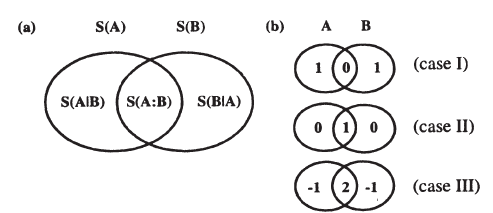
\includegraphics[width=0.9\textwidth]{gambar/DIAGRAM/diagram2.png}
                \captionsetup{font=tiny, justification=justified}
                \captionof{figure}{Contoh caption: diagram entropi sistem
                dua-qubit. Nomor otomatis \textit{slide.urutan}.}
                \label{fig:contoh}
            \end{figure}
            {\tiny Rujuk dengan
            \code{Gambar~\ref{fig:contoh}} $\rightarrow$
            Gambar~\ref{fig:contoh}.}
        \end{column}

        \begin{column}{0.52\textwidth}
            % --- TABEL PROFESIONAL (booktabs) --------------------------
            \begin{table}
                \centering
                {\tiny
                \begin{tabular}{llc}
                    \toprule                              % garis atas
                    \textbf{Perintah} & \textbf{Hasil} & \textbf{Ket.} \\
                    \midrule                              % garis tengah
                    \code{\sigma_x} & $\sigma_x$ & Pauli-X \\
                    \code{\otimes}   & $\otimes$  & tensor  \\
                    \code{\dagger}   & $\dagger$  & adjoint \\
                    \bottomrule                           % garis bawah
                \end{tabular}}
                \captionof{table}{Contoh tabel \textit{booktabs}.}
                \label{tab:contoh}
            \end{table}

            % --- PERSAMAAN BERLABEL ------------------------------------
            %  \label{eq:...} lalu rujuk: Persamaan~\ref{eq:vonneumann}
            \begin{equation}
                S(\rho) = -\Tr\!\left(\rho \log \rho\right)
                \label{eq:vonneumann}
            \end{equation}
            {\tiny Persamaan~\ref{eq:vonneumann} = entropi von Neumann.}
        \end{column}
    \end{columns}
\end{frame}

%---------------------------------------------------------------------
%  CONTOH 3 — NOTASI KUANTUM (DIRAC) & TULISAN MATEMATIKA
%---------------------------------------------------------------------
%  Makro notasi tersedia di ppt.sty bagian [8]; paket braket menyediakan
%  \ket, \bra, \Braket. Prinsip penulisan:
%    * vektor keadaan selalu \ket{...}   ->  |psi>
%    * dual (transpose konjugat) \bra{...}
%    * proyektor \ketbra{a}{b}           ->  |a><b|
%    * operator ditandai "topi": \hat{U}
\begin{frame}
    \frametitle{Cheatsheet Notasi Kuantum}
    \begin{columns}[T]
        \begin{column}{0.48\textwidth}
            {\small\textbf{Keadaan \& operator}}
            {\tiny
            \begin{itemize}\justifying
                \item[$\Rightarrow$] Qubit:
                      $\ket{0}=\begin{bmatrix}1\\0\end{bmatrix}$,
                      $\ket{1}=\begin{bmatrix}0\\1\end{bmatrix}$
                \item[$\Rightarrow$] Superposisi:
                      $\ket{\psi}=\alpha\ket{0}+\beta\ket{1}$,
                      $|\alpha|^2+|\beta|^2=1$
                \item[$\Rightarrow$] Bell/EPR:
                      $\ket{\psi_{AB}}=\tfrac{1}{\sqrt{2}}(\ket{00}+\ket{11})$
                \item[$\Rightarrow$] Proyektor: $\ketbra{0}{0}$,
                      $\ketbra{1}{1}$
                \item[$\Rightarrow$] Operator: $\hat{U}\hat{U}^\dagger=\hat{I}$
            \end{itemize}}
        \end{column}
        \begin{column}{0.48\textwidth}
            {\small\textbf{Matriks densitas \& entropi}}
            {\tiny
            \begin{itemize}\justifying
                \item[$\Rightarrow$] Campuran:
                      $\rho=\sum_i p_i\,\ketbra{\psi_i}{\psi_i}$
                \item[$\Rightarrow$] Matriks gabungan:
                      $\rho_{AB}=\rho_A\otimes\rho_B$
                \item[$\Rightarrow$] Jejak (trace):
                      $\Tr(\rho)=1$;
                      $\Tr_B(\rho_{AB})=\rho_A$
                \item[$\Rightarrow$] Entropi:
                      $S(\rho)=-\Tr(\rho\log\rho)$
                \item[$\Rightarrow$] Kondisional:
                      $S(A|B)=S(AB)-S(B)$ (bisa negatif!)
            \end{itemize}}
        \end{column}
    \end{columns}
\end{frame}

%---------------------------------------------------------------------
%  CONTOH 4 — MENULIS KODE PROGRAM (LISTINGS)
%---------------------------------------------------------------------
\begin{frame}[fragile]   % [fragile] WAJIB jika slide berisi lstlisting
    \frametitle{Menampilkan Kode Program}
    \begin{columns}[T]
        \begin{column}{0.48\textwidth}
            {\tiny Gaya kode diatur di \code{ppt.sty} bagian [7].
                   Selalu tambahkan opsi \code{[fragile]} pada frame
                   yang memuat \code{lstlisting}.}
            \begin{lstlisting}[language=Python,basicstyle=\ttfamily\scriptsize]
# Contoh simulasi qubit (Python)
import numpy as np
I = np.eye(2)          # matriks identitas
X = np.array([[0, 1],
              [1, 0]]) # Pauli-X
rho = 0.5*(I + X)      # matriks densitas
print(np.trace(rho))   # Tr(rho) = 1
            \end{lstlisting}
        \end{column}
        \begin{column}{0.48\textwidth}
            \begin{lstlisting}[language=Matlab,basicstyle=\ttfamily\scriptsize]
% Contoh kanal depolarizing (MATLAB)
p  = 0.05;              % prob. depolarisasi
I2 = eye(2);
rho_i = [0.5 0; 0 0.5];
rho  = p*(I2/2) + (1-p)*rho_i;
            \end{lstlisting}
            {\tiny Kode inline: gunakan \code{\code{...}},
                   contoh: \code{np.trace(rho)}.}
        \end{column}
    \end{columns}
\end{frame}

%---------------------------------------------------------------------
%  CONTOH 5 — KUTIPAN, FOOTNOTE & BLOK
%---------------------------------------------------------------------
\begin{frame}
    \frametitle{Kutipan Pustaka \& Blok Informasi}
    \begin{columns}[T]
        \begin{column}{0.48\textwidth}
            \begin{exampleblock}{Kutipan dari bib.bib}
                {\small
                \begin{itemize}\justifying
                    \item Nomor biasa: entropi kuantum
                          \cite{barnett2009quantum}.
                    \item Footnote lengkap (pertama kali):\
                          lihat catatan kaki bawah slide.
                    \item Footnote ringkas (kutipan berikutnya):\
                          juga di catatan kaki.
                \end{itemize}}
            \end{exampleblock}
            {\tiny Entri pustaka ditulis di \code{bib.bib}.}
        \end{column}
        \begin{column}{0.48\textwidth}
            \begin{alertblock}{Alert block --- hal penting}
                {\small Dipakai untuk peringatan/kesimpulan kunci.}
            \end{alertblock}
            \begin{block}{Block biasa}
                {\small Definisi, catatan, atau langkah analisis.}
            \end{block}
            {\tiny Footnote biasa juga bisa: teks\footnote{Contoh
                   footnote langsung tanpa berkas pustaka.}}
        \end{column}
    \end{columns}
    % CATATAN PENTING: footnote/citasi ber-footnote (irstcite dsb.)
    % dipanggil di LEVEL FRAME (di luar columns) agar lebarnya terpotok
    % dan tidak meluber keluar slide.
    \vspace{-0.1cm}{\tiny \firstcite{cerf1997negative};
     kutip ulang \secondcite{cerf1997negative}.}
\end{frame}
 di main.tex saat presentasi.
%
%  TIPS: untuk menuliskan nama perintah/kode di dalam teks, gunakan
%  \code{...} (makro bawaan ppt.sty) — contoh \code{\frac{a}{b}}.
%=====================================================================

%---------------------------------------------------------------------
%  CONTOH 1 — STRUKTUR DASAR SLIDE & TEKS
%---------------------------------------------------------------------
\section{PANDUAN PENGGUNAAN}

\begin{frame}
    \frametitle{Cara Membuat Slide Baru}   % judul yang tampil di batang atas

    % --- Struktur minimum sebuah slide ----------------------------
    %  \begin{frame}
    %      \frametitle{Judul Slide Anda}
    %      isi slide ...
    %  \end{frame}
    %  Letakkan \section{NAMA BAGIAN} SEBELUM \begin{frame} agar
    %  slide masuk ke navigasi atas dan slide OUTLINE.

    \begin{columns}[T]          % [T] = rata atas antar kolom
        \begin{column}{0.48\textwidth}   % lebar kolom (48% teks)
            \begin{block}{Penekanan teks}
                \footnotesize
                \begin{itemize}
                    \item \textbf{tebal}  : \code{\textbf{tebal}}
                    \item \textit{miring} : \code{\textit{miring}}
                    \item \alert{merah}   : \code{\alert{merah}}
                    \item \textcolor{telu}{merah Telkom}:\\
                          \code{\textcolor{telu}{...}}
                \end{itemize}
            \end{block}
        \end{column}

        \begin{column}{0.48\textwidth}
            \begin{block}{Ukuran font \& perataan}
                \footnotesize
                \begin{itemize}
                    \item[\textcolor{scisGold}{$\Rightarrow$}] Urut kecil:
                          \code{\tiny < \small < \normalsize}
                    \item[\textcolor{scisGold}{$\Rightarrow$}] Rata kiri-kanan:
                          tulis \code{\justifying} (paket ragged2e)
                    \item[\textcolor{scisGold}{$\Rightarrow$}] Daftar bertingkat:
                          \code{\item} di dalam \code{\item}
                    \item[\textcolor{scisGold}{$\Rightarrow$}] Panah khusus:
                          \code{\item[$\Rightarrow$]}
                \end{itemize}
            \end{block}
        \end{column}
    \end{columns}
\end{frame}

%---------------------------------------------------------------------
%  CONTOH 2 — GAMBAR, TABEL & PERSAMAAN
%---------------------------------------------------------------------
\begin{frame}
    \frametitle{Memasukkan Gambar, Tabel \& Persamaan}
    \begin{columns}[T]
        \begin{column}{0.46\textwidth}
            % --- GAMBAR + CAPTION + LABEL -----------------------------
            %  \label wajib UNIK; rujuk dengan Gambar~\ref{fig:contoh}
            \begin{figure}
                \centering
                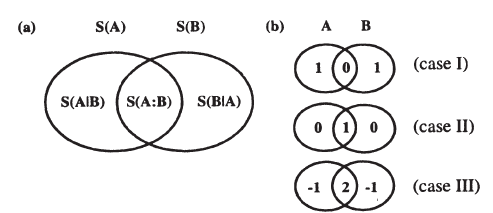
\includegraphics[width=0.9\textwidth]{gambar/DIAGRAM/diagram2.png}
                \captionsetup{font=tiny, justification=justified}
                \captionof{figure}{Contoh caption: diagram entropi sistem
                dua-qubit. Nomor otomatis \textit{slide.urutan}.}
                \label{fig:contoh}
            \end{figure}
            {\tiny Rujuk dengan
            \code{Gambar~\ref{fig:contoh}} $\rightarrow$
            Gambar~\ref{fig:contoh}.}
        \end{column}

        \begin{column}{0.52\textwidth}
            % --- TABEL PROFESIONAL (booktabs) --------------------------
            \begin{table}
                \centering
                {\tiny
                \begin{tabular}{llc}
                    \toprule                              % garis atas
                    \textbf{Perintah} & \textbf{Hasil} & \textbf{Ket.} \\
                    \midrule                              % garis tengah
                    \code{\sigma_x} & $\sigma_x$ & Pauli-X \\
                    \code{\otimes}   & $\otimes$  & tensor  \\
                    \code{\dagger}   & $\dagger$  & adjoint \\
                    \bottomrule                           % garis bawah
                \end{tabular}}
                \captionof{table}{Contoh tabel \textit{booktabs}.}
                \label{tab:contoh}
            \end{table}

            % --- PERSAMAAN BERLABEL ------------------------------------
            %  \label{eq:...} lalu rujuk: Persamaan~\ref{eq:vonneumann}
            \begin{equation}
                S(\rho) = -\Tr\!\left(\rho \log \rho\right)
                \label{eq:vonneumann}
            \end{equation}
            {\tiny Persamaan~\ref{eq:vonneumann} = entropi von Neumann.}
        \end{column}
    \end{columns}
\end{frame}

%---------------------------------------------------------------------
%  CONTOH 3 — NOTASI KUANTUM (DIRAC) & TULISAN MATEMATIKA
%---------------------------------------------------------------------
%  Makro notasi tersedia di ppt.sty bagian [8]; paket braket menyediakan
%  \ket, \bra, \Braket. Prinsip penulisan:
%    * vektor keadaan selalu \ket{...}   ->  |psi>
%    * dual (transpose konjugat) \bra{...}
%    * proyektor \ketbra{a}{b}           ->  |a><b|
%    * operator ditandai "topi": \hat{U}
\begin{frame}
    \frametitle{Cheatsheet Notasi Kuantum}
    \begin{columns}[T]
        \begin{column}{0.48\textwidth}
            {\small\textbf{Keadaan \& operator}}
            {\tiny
            \begin{itemize}\justifying
                \item[$\Rightarrow$] Qubit:
                      $\ket{0}=\begin{bmatrix}1\\0\end{bmatrix}$,
                      $\ket{1}=\begin{bmatrix}0\\1\end{bmatrix}$
                \item[$\Rightarrow$] Superposisi:
                      $\ket{\psi}=\alpha\ket{0}+\beta\ket{1}$,
                      $|\alpha|^2+|\beta|^2=1$
                \item[$\Rightarrow$] Bell/EPR:
                      $\ket{\psi_{AB}}=\tfrac{1}{\sqrt{2}}(\ket{00}+\ket{11})$
                \item[$\Rightarrow$] Proyektor: $\ketbra{0}{0}$,
                      $\ketbra{1}{1}$
                \item[$\Rightarrow$] Operator: $\hat{U}\hat{U}^\dagger=\hat{I}$
            \end{itemize}}
        \end{column}
        \begin{column}{0.48\textwidth}
            {\small\textbf{Matriks densitas \& entropi}}
            {\tiny
            \begin{itemize}\justifying
                \item[$\Rightarrow$] Campuran:
                      $\rho=\sum_i p_i\,\ketbra{\psi_i}{\psi_i}$
                \item[$\Rightarrow$] Matriks gabungan:
                      $\rho_{AB}=\rho_A\otimes\rho_B$
                \item[$\Rightarrow$] Jejak (trace):
                      $\Tr(\rho)=1$;
                      $\Tr_B(\rho_{AB})=\rho_A$
                \item[$\Rightarrow$] Entropi:
                      $S(\rho)=-\Tr(\rho\log\rho)$
                \item[$\Rightarrow$] Kondisional:
                      $S(A|B)=S(AB)-S(B)$ (bisa negatif!)
            \end{itemize}}
        \end{column}
    \end{columns}
\end{frame}

%---------------------------------------------------------------------
%  CONTOH 4 — MENULIS KODE PROGRAM (LISTINGS)
%---------------------------------------------------------------------
\begin{frame}[fragile]   % [fragile] WAJIB jika slide berisi lstlisting
    \frametitle{Menampilkan Kode Program}
    \begin{columns}[T]
        \begin{column}{0.48\textwidth}
            {\tiny Gaya kode diatur di \code{ppt.sty} bagian [7].
                   Selalu tambahkan opsi \code{[fragile]} pada frame
                   yang memuat \code{lstlisting}.}
            \begin{lstlisting}[language=Python,basicstyle=\ttfamily\scriptsize]
# Contoh simulasi qubit (Python)
import numpy as np
I = np.eye(2)          # matriks identitas
X = np.array([[0, 1],
              [1, 0]]) # Pauli-X
rho = 0.5*(I + X)      # matriks densitas
print(np.trace(rho))   # Tr(rho) = 1
            \end{lstlisting}
        \end{column}
        \begin{column}{0.48\textwidth}
            \begin{lstlisting}[language=Matlab,basicstyle=\ttfamily\scriptsize]
% Contoh kanal depolarizing (MATLAB)
p  = 0.05;              % prob. depolarisasi
I2 = eye(2);
rho_i = [0.5 0; 0 0.5];
rho  = p*(I2/2) + (1-p)*rho_i;
            \end{lstlisting}
            {\tiny Kode inline: gunakan \code{\code{...}},
                   contoh: \code{np.trace(rho)}.}
        \end{column}
    \end{columns}
\end{frame}

%---------------------------------------------------------------------
%  CONTOH 5 — KUTIPAN, FOOTNOTE & BLOK
%---------------------------------------------------------------------
\begin{frame}
    \frametitle{Kutipan Pustaka \& Blok Informasi}
    \begin{columns}[T]
        \begin{column}{0.48\textwidth}
            \begin{exampleblock}{Kutipan dari bib.bib}
                {\small
                \begin{itemize}\justifying
                    \item Nomor biasa: entropi kuantum
                          \cite{barnett2009quantum}.
                    \item Footnote lengkap (pertama kali):\
                          lihat catatan kaki bawah slide.
                    \item Footnote ringkas (kutipan berikutnya):\
                          juga di catatan kaki.
                \end{itemize}}
            \end{exampleblock}
            {\tiny Entri pustaka ditulis di \code{bib.bib}.}
        \end{column}
        \begin{column}{0.48\textwidth}
            \begin{alertblock}{Alert block --- hal penting}
                {\small Dipakai untuk peringatan/kesimpulan kunci.}
            \end{alertblock}
            \begin{block}{Block biasa}
                {\small Definisi, catatan, atau langkah analisis.}
            \end{block}
            {\tiny Footnote biasa juga bisa: teks\footnote{Contoh
                   footnote langsung tanpa berkas pustaka.}}
        \end{column}
    \end{columns}
    % CATATAN PENTING: footnote/citasi ber-footnote (irstcite dsb.)
    % dipanggil di LEVEL FRAME (di luar columns) agar lebarnya terpotok
    % dan tidak meluber keluar slide.
    \vspace{-0.1cm}{\tiny \firstcite{cerf1997negative};
     kutip ulang \secondcite{cerf1997negative}.}
\end{frame}
